\setlength{\columnsep}{3pt}
\begin{flushleft}
	\bigskip
	\begin{itemize}
		\item Files has following attributes as metadata:
			\begin{figure}[h!]
				\centering
				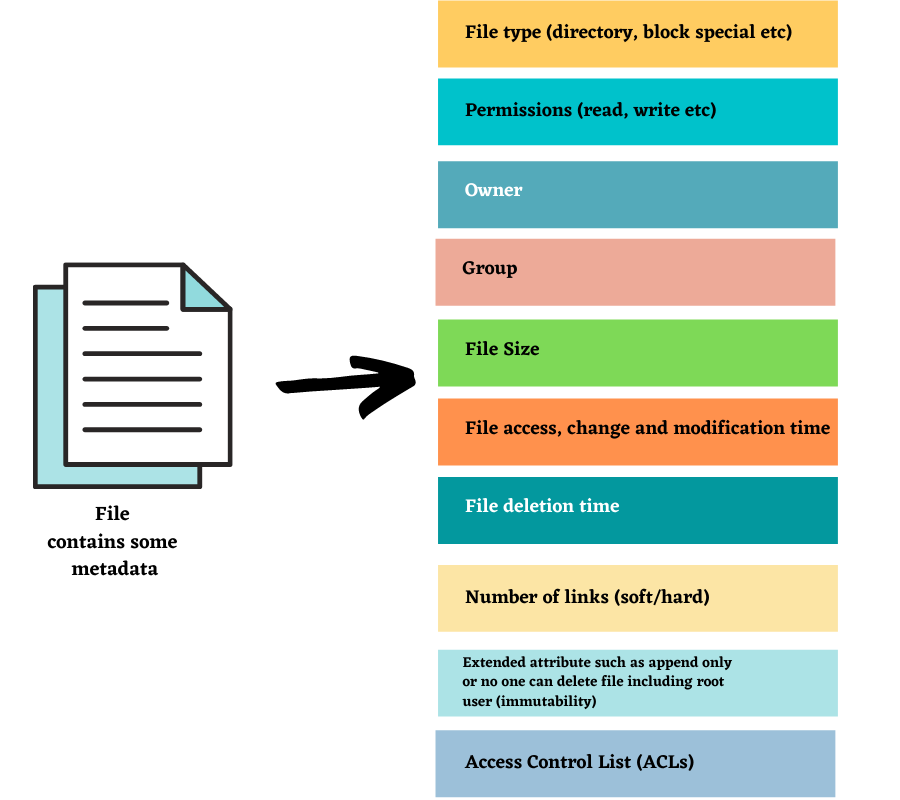
\includegraphics[scale=.6]{content/chapter8/images/meta.png}
				\caption{File attributes}
				\label{fig:File_attributes}
			\end{figure}
		\item All the above information is stored in an \textbf{inode}. 
		\item The inode stands for \textbf{index node} (also called as index node).
	\end{itemize}
	
\end{flushleft}

\newpage

